%%%%%%%%% begin snippet
%% You need to add the package "tabularx".
%% Place the snippet right after \begin{document}

% need tabularx
\documentclass{article}
\usepackage{tabularx}
\usepackage{graphicx}
\usepackage{pdfpages}
\usepackage{listings}
\usepackage{subcaption}
\usepackage{verbatim}

\begin{document}
    \begin{titlepage}
           \begin{center}
                 \begin{huge}
                       %% Update assignment number here
                       \textbf{Assignment 4}
                 \end{huge}
           \end{center}

           \begin{center}
                 \begin{large}
                       Machine Learning 1, SS23
                 \end{large}
           \end{center}

           \begin{center}
                \begin{tabularx}{\textwidth}{|>{\hsize=.33\hsize}X|>{\hsize=.33\hsize}X|>{\hsize=.33\hsize}X|}

                       \hline
                       \multicolumn{3}{|c|}{\textbf{Team Members}} \\
                       \hline
                       Last name & First name & Matriculation Number \\
                       \hline
                       Grassl & Ifeoma & 12011965 \\
                       \hline
                       Royer & Christoph & 12004184 \\
                       \hline

                \end{tabularx}
           \end{center}

    \end{titlepage}

    \section{Maximum Likelihood Estimation}
    // todo

    \section{K-means. Expectation-Maximization Algorithm}
    \subsection{K-means Algorithm}
    \label{subseq:kmeans}
    \textit{See implementation in} \texttt{k\_means.py}

    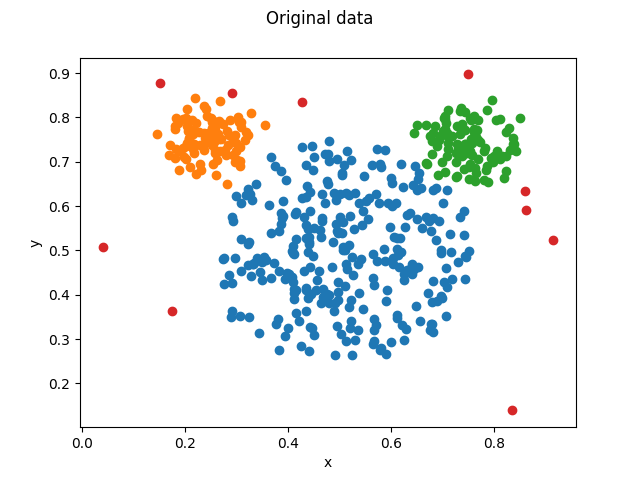
\includegraphics[width=\textwidth/2]{plots/mickey_original} \\
    The original data shows three nearly circular clusters with a few outliers.

    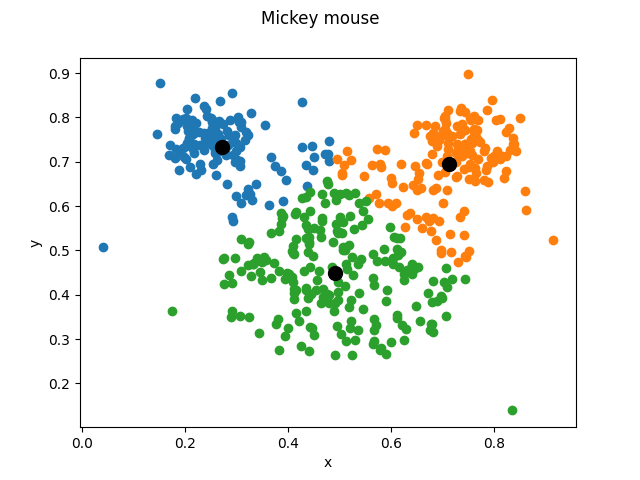
\includegraphics[width=\textwidth / 2]{plots/mickey_k3}
    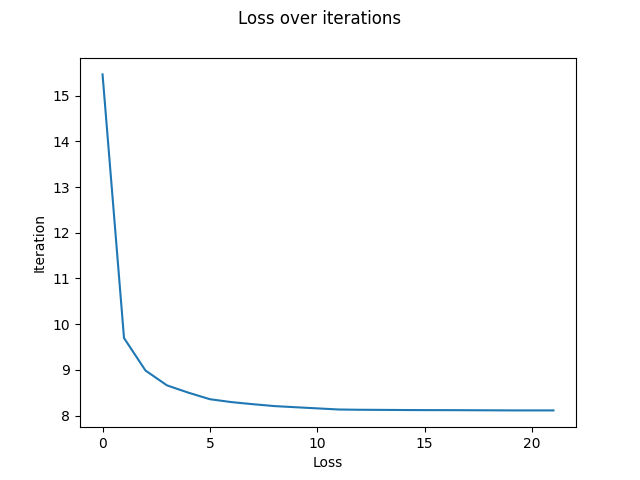
\includegraphics[width=\textwidth / 2]{plots/mickey_k3_loss} \\
    When compared to the original data, a K-means with $K=3$ shows some problems.
    Some of the samples of the main cluster are attributed to the smaller, upper clusters.
    This is because though they would fit better with the big cluster, they are technically nearer to the smaller centroids.

    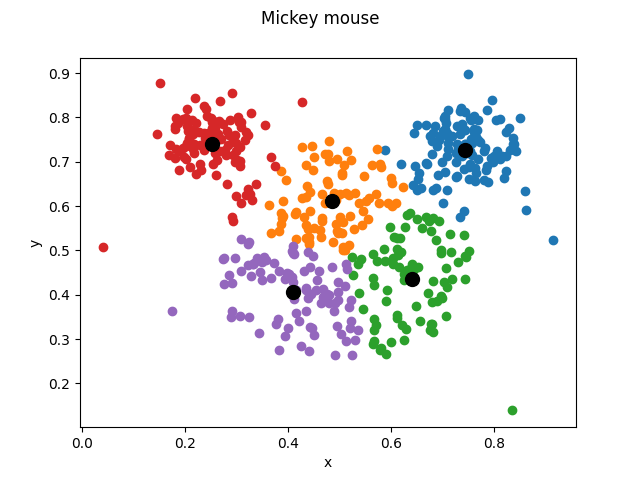
\includegraphics[width=\textwidth / 2]{plots/mickey_k5}
    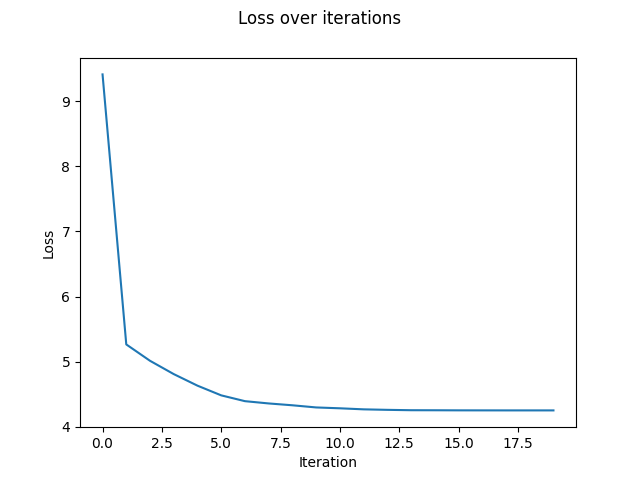
\includegraphics[width=\textwidth / 2]{plots/mickey_k5_loss}
    When setting $K=5$, the problem of the small clusters bleeding into the big one is mostly fixed.
    But now one would manually have to stitch together the three centroids that all take up some of the space in the big cluster.

    \subsection{Expectation-Maximization Algorithm}
    \textit{See implementation in} \texttt{em.py}

    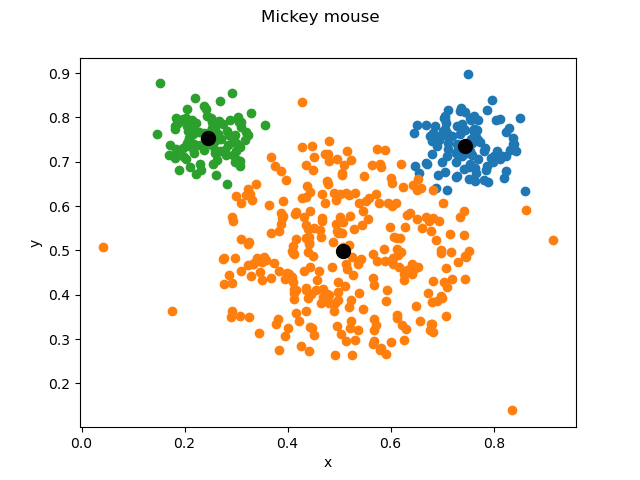
\includegraphics[width=\textwidth / 2]{plots/mickey_em3}
    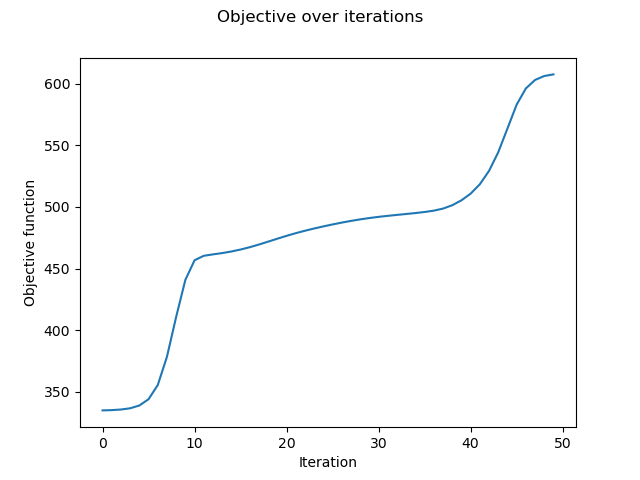
\includegraphics[width=\textwidth / 2]{plots/mickey_em3_likelihood}
    Compared to the original data (see \ref{subseq:kmeans}), the EM-algorithm provides a very good result.
    Nearly all of the points are correclty classified, although the algorithm still cannot identify the outliers as such.
    We also see none of the problems the K-means algorithm had, where parts of the big cluster were assigned to one of the smaller clusters.

    This is also reflected in the final values of $\pi$.
    We can see clearly that the bigger cluster got a bigger weight, while the two smaller clusters have a similar, smaller weight.\\
    Inital value of $\pi$: \texttt{Init pi: [0.33333333 0.33333333 0.33333333]}\\
    Final value of $\pi$: \texttt{Pi: [0.60036228 0.20177808 0.19785964]}

    \subsection{Summary and comparison of two algorithms}
    //todo

    \section{Image segmentation using K-means -- Code analysis}
    // todo


\end{document}

%%%%%%%%% end snippet
